\documentclass[10pt]{article}
\usepackage[utf8]{inputenc}

\usepackage{natbib}
\usepackage{setspace}
\usepackage{wrapfig}
\usepackage{graphicx}
\usepackage{caption}
\usepackage{subfig}
\usepackage{hyperref}
\usepackage{url}
\usepackage{geometry}
\usepackage{amsmath}
\usepackage{amssymb}

\geometry{margin=1in}
\onehalfspacing

\begin{document}

\begin{center}
  2LT Mahdi Al-Husseini $\bullet$ MEDEVAC Dispatch Policy NetLogo Simulation Technical Report $\bullet$ 1AUG18
\end{center}

\section{Introduction and Background}
Medical evacuation (MEDEVAC) air ambulance asset dispatch strategy directly affects the survival of transported casualties. The negative relationship between MEDEVAC response time and patient survival is well-documented in the academic literature. Casualties are categorized by severity of injury into either A. Urgent, B. Priority, or C. Routine. Notably, MEDEVAC response time thresholds (RTT) for evacuation of Urgent patients differs in the US and NATO. RTT in the US is sixty minutes, whereas RTT in NATO is ninety minutes. This NetLogo simulation builds on the work of Keneally, Robbins, and Lunday$^3$, who developed a markov decision process model to optomize the MEDEVAC dispatch strategy in Southern Afghanistan during Operation Enduring Freedom. The presented NetLogo simulation was developed while attending the Army Medical Department (AMEDD) Basic Officer Leadership Course (BOLC).
\\~\\
Three dispatch strategies were examined: intra-zone, myopic, and optimal. Intra-zone dispatching limits MEDEVAC assets to their assigned zones, which in this simulation, represented the Nimroz, Helmand, Kandahar, and Zabul provinces of Southern Afghanistan. Myopic dispatching selects the MEDEVAC asset closest to the casualty, regardless of severity of injury. Optimal dispatching takes into account severity of injury as well as relative zone violence levels. The NetLogo simulation was outfitted with each dispatching strategy, and run for 100 simulation days, 400 times each, for a total of 120,000 days of simulation data. The total utility was then compared across dispatch policies. The total utility function quantifies the life saving capacity of each dispatch policy by giving weight to response times for urgent and priority patients below their respective RTTs.
\section{Parameters, Metrics, Functions}
$RT$ = $f(EC, CL, PAE, v_{UH-60}, D, A, L, U, CIP, n_{MED}, n_{MTF}, n_{EVE},  GIS, DS)$ \\~\\
RT: response time,
EC: event classification probabilities,
CL: casualty load probabilities,
PAE: armed escort probability,
$v_{UH-60}$: UH-60 nautical speed,
D: average dispatch time,
A: average armed escort delay,
L: average casualty load time,
U: average casualty unload time,
CIP: casualty incidence rate by province,
n$_{MED}$: number of MEDEVACS in area,
n$_{MTF}$: number of MTFs in area,
n$_{EVE}$: number of events in area over time,
GIS: graphical information system (GIS) data on Nimroz, Helmand, Kandahar, and Zabul provinces,
DS: dispatching strategy
\\~\\
$TU_t$ = $f(RT, RTT, t, EC, CL)$ \\~\\
RT: response time,
RTT: response time threshold (RTT),
t: time elapsed,
EC: event classification probabilities,
CL: casualty load probabilities
\section{Analysis and Results}
\\
\begin{figure}[h!]
    \centering
    \subfloat[]{{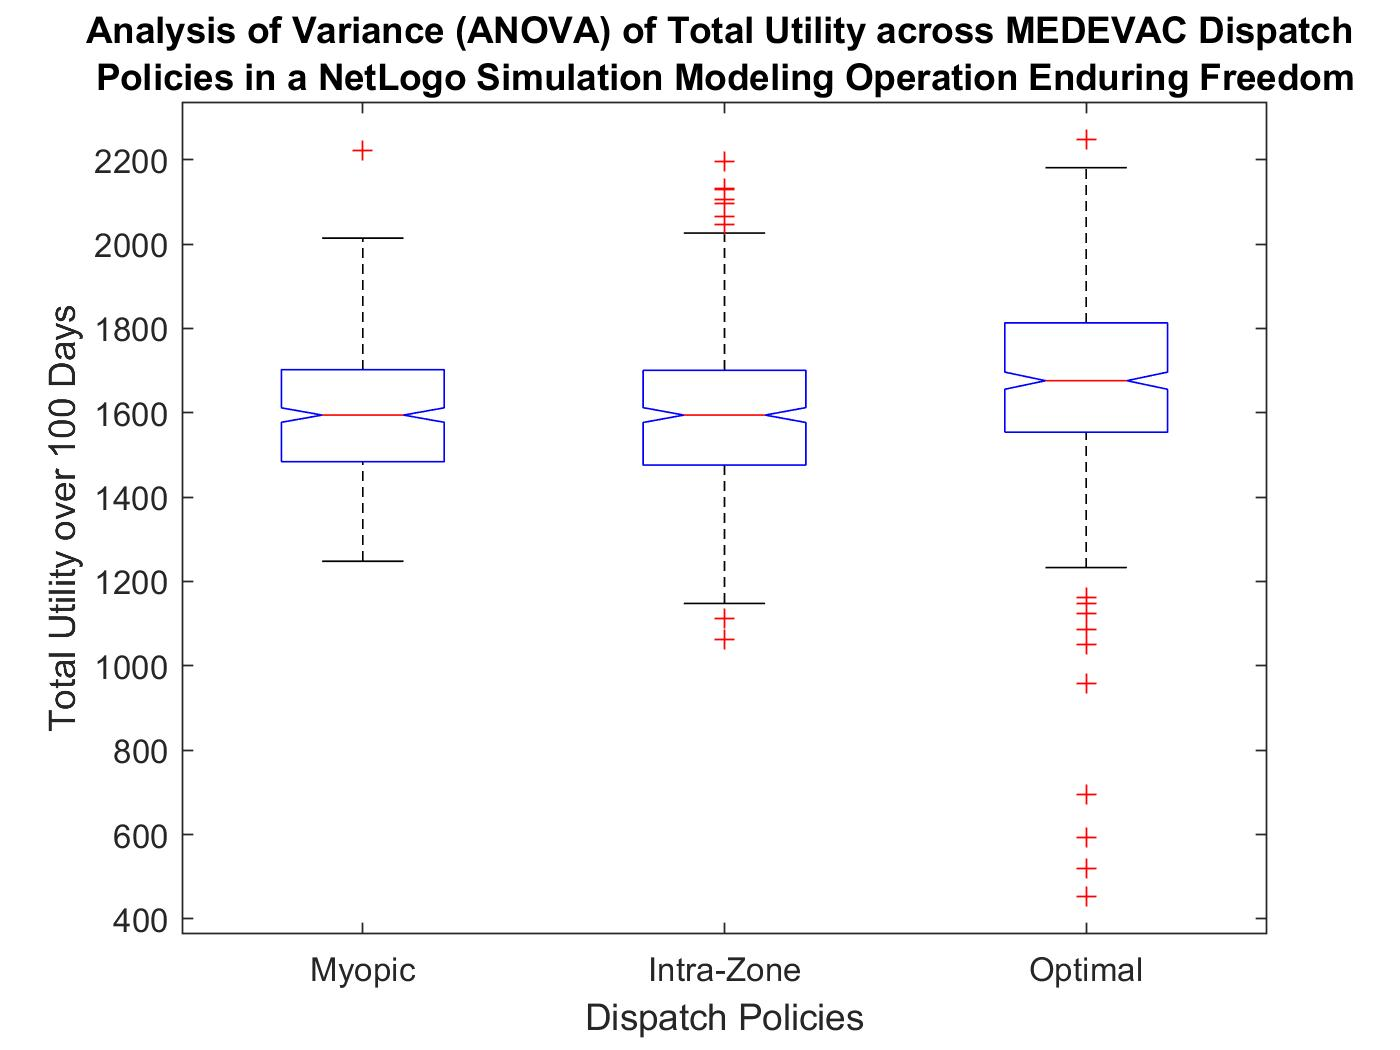
\includegraphics[width=7cm]{ANOVA.jpg} }}
    \qquad
    \subfloat[]{{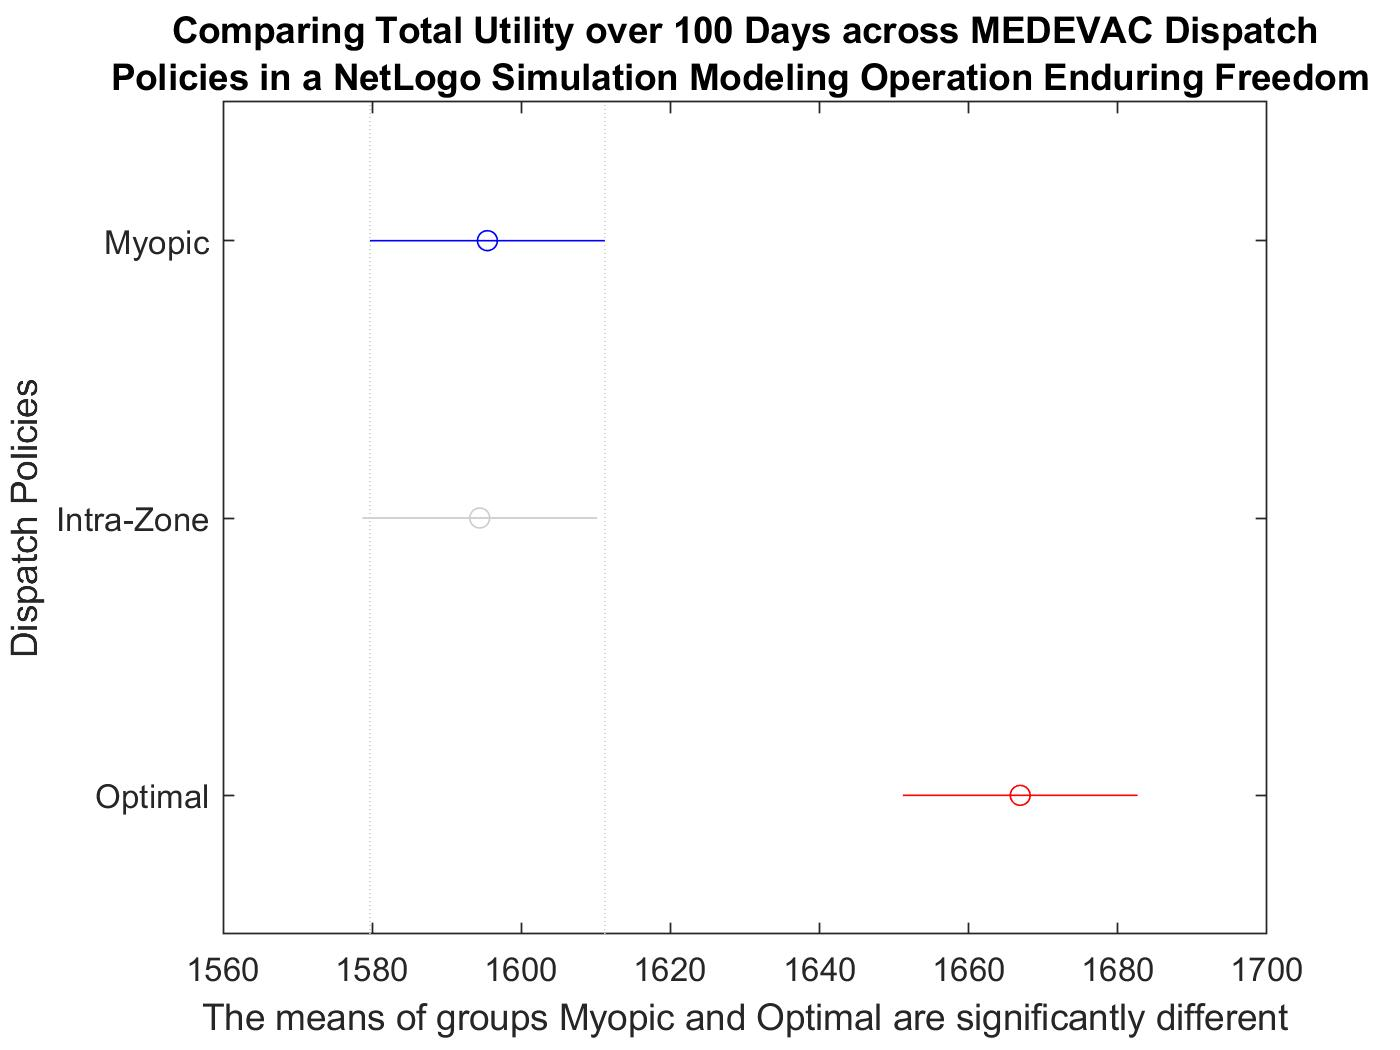
\includegraphics[width=7cm]{multcompare.jpg} }}
    \caption{}
    \label{}
\end{figure}
\\
As shown in Figure 1, the average total utility across 100 days where n = 400 for an optimal policy was shown to be significantly greater than that of both myopic and intra-zone policies, while no significant difference was shown between the latter two. The total utility across 100 days for an optimal policy was found to be 1595.46 with a standard deviation of 157.62. The total utility across 100 days for a myopic policy was found to be 1594.43 with a standard deviation of 221.83. The total utility across 100 days for an optimal policy was found to be 1666.91 with a standard deviation of 185.06.
\section{References}
\noindent
\hangindent=2em
Aksyonov, K. A., et al. "Development of the MEDEVAC operations simulation 	model." Control And Decision Conference (CCDC), 2017 29th Chinese. 	IEEE, 2017.
\par
\noindent
\hangindent=2em
Jenkins, Phillip R. Using Markov Decision Processes with Heterogeneous 	Queueing Systems to Examine Military MEDEVAC Dispatching Policies. No. 	AFIT-ENS-MS-17-M-137. Air Force Institute of Technology WPAFB United 	States, 2017.
\par
\noindent
\hangindent=2em
Keneally, Sean K., Matthew J. Robbins, and Brian J. Lunday. "A markov 	decision process model for the optimal dispatch of military medical 	evacuation assets." Health care management science 19.2 (2016): 111-	129.
\par
\noindent
\hangindent=2em
Rettke, Aaron J., Matthew J. Robbins, and Brian J. Lunday. "Approximate 	dynamic programming for the dispatch of military medical evacuation 	assets." European Journal of Operational Research 254.3 (2016): 824-839.
\section{Link}
Download this NetLogo simulation and the corresponding presentation at:\\
http://www.mahdial-husseini.com/personal$\_$project$\_$pages/dispatchsim.html
\end{document}
